\chapter{Termodinámica de las pilas electroquímicas}\label{ch:b2:cell-thermodynamics}

Un autobús de pila de combustible de hidrógeno lleva una pila de unos cientos de celdas finas. En cada una,
el hidrógeno y el oxígeno del aire se combinan dando agua sin llama, y la
energía sale en forma de corriente eléctrica. Dos números gobiernan una pila así, y
ambos salen directamente de las tablas de \omterm{def:b2:reaction-free-energy:gibbs-energy}{energías de Gibbs}: ninguna celda puede dar más de
\qty{1.23}{V}, y ninguna pila de combustible, por perfecta que sea, convierte toda la energía de su
hidrógeno en trabajo eléctrico. Este capítulo relaciona la tensión de una pila con
la \omterm{def:b2:reaction-free-energy:gibbs-energy}{energía de Gibbs} de su reacción, deduce la ecuación de Nernst usada desde el
volumen del primer año, y lee entropías y \omterm{def:b2:reaction-enthalpy:reaction-quantity}{entalpías de reacción} en un voltímetro
y un termómetro.

\begin{recall}
El volumen del primer año: pilas, semipilas, ánodo y cátodo, puente salino, tensión
de la pila, potencial de electrodo, potencial estándar y electrodo estándar de
hidrógeno, la ecuación de Nernst (admitida allí), constantes de equilibrio a partir de
potenciales. \Cref{ch:b2:reaction-free-energy}: $\Delta_r G$, $\Delta_r G^\circ$
y $\Delta_r G = \Delta_r G^\circ + RT\ln Q$; el criterio de evolución.
\Cref{ch:b2:chemical-potential}: actividades. El volumen escolar: la electrólisis.
\end{recall}

\begin{omfigure}
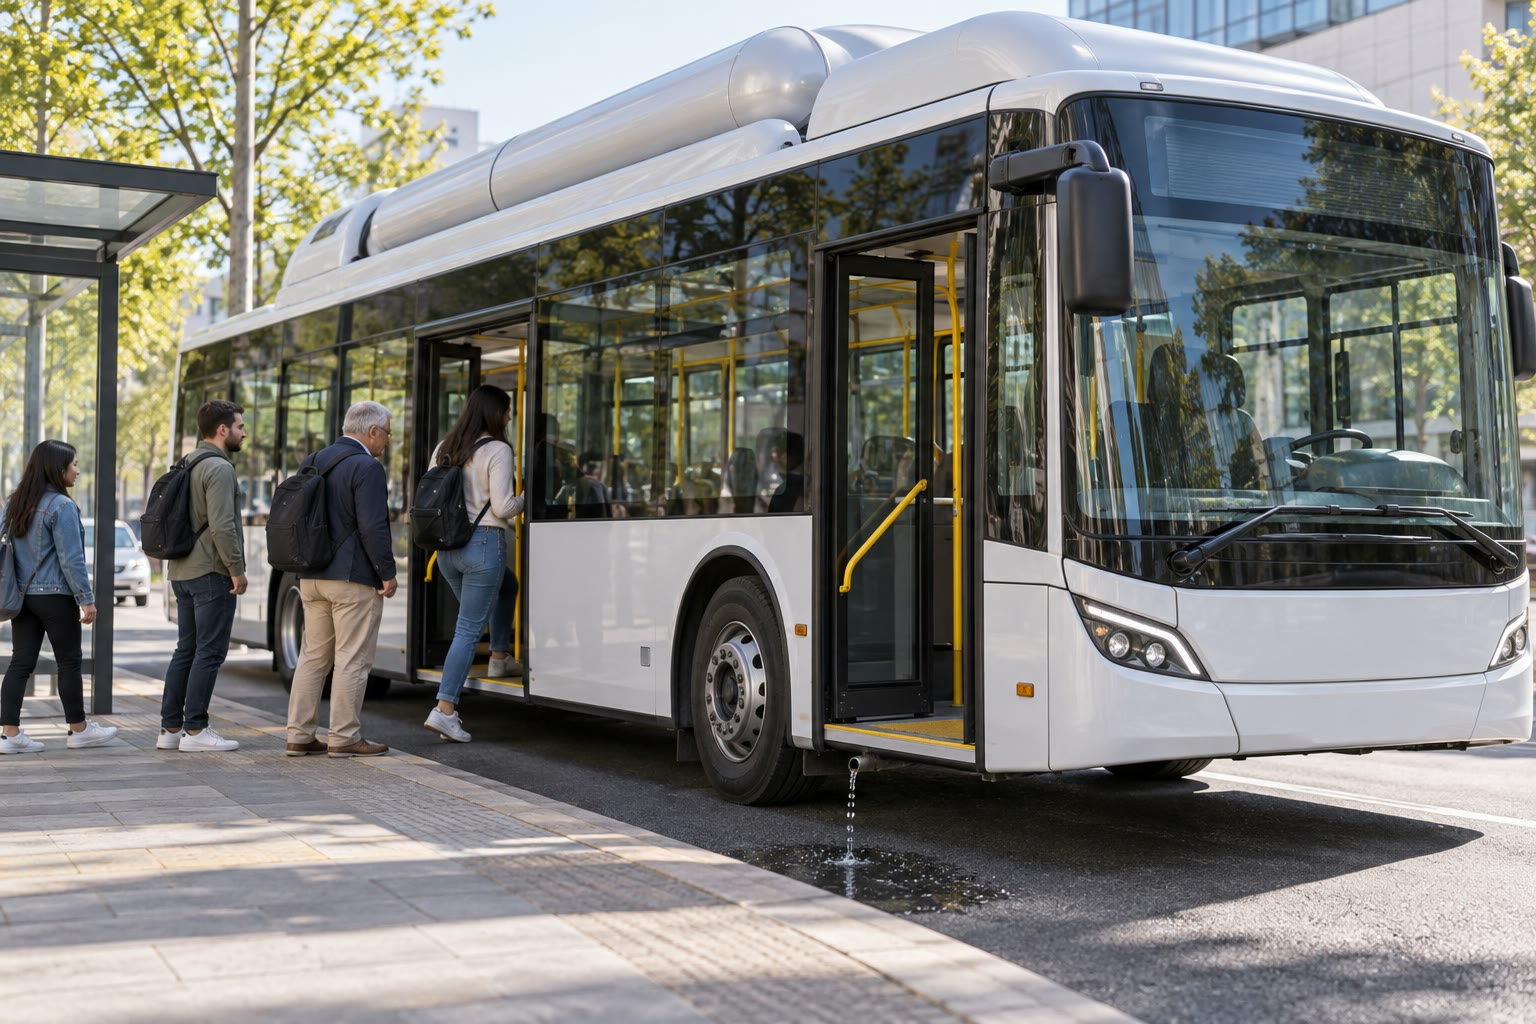
\includegraphics[width=0.62\linewidth]{images/book3/ai/b2-09-fuel-cell-bus.jpg}

{\small Un autobús de pila de combustible de hidrógeno en una parada: los depósitos de hidrógeno están bajo el
carenado del techo, y el único escape es agua, que gotea bajo el autobús.}
\end{omfigure}

\section{Trabajo eléctrico y constante de Faraday}

\begin{definition}[Constante de Faraday]\label{def:b2:cell-thermodynamics:faraday}
La \emph{constante de Faraday}\index{constante de Faraday} es la carga eléctrica de
un mol de cargas elementales, $F = N_A e = \qty{96485.33}{C/mol}$.
% ledger: const:F
\end{definition}

\begin{proposition}[Carga transferida]\label{prop:b2:cell-thermodynamics:charge}
Si la reacción de una pila, escrita con $n$ electrones intercambiados, avanza en
$\Delta\xi$, la carga que circula por el circuito exterior es $Q =
nF\,\Delta\xi$.
\end{proposition}

\begin{proof}
Un avance $\Delta\xi$ transfiere $n\,\Delta\xi$ moles de electrones del
ánodo al cátodo a través del hilo, cada uno de carga $e$ en valor absoluto:
$Q = n\,\Delta\xi\,N_A e$.
\end{proof}

Cuando una carga $Q$ recorre un circuito impulsada por una tensión $U$, el trabajo
que recibe el circuito es $QU$. Visto desde la pila, que suministra ese trabajo,
el trabajo eléctrico que recibe es $\delta W_{\text{el}} = -U\,\delta Q = -nFU\,
d\xi$.

\begin{omfigure}
\begin{tikzpicture}[font=\small, >={Stealth}]
  \draw[thick, rounded corners, fill=omDef!8] (0,0) rectangle (3.2,2.2);
  \node[align=center] at (1.6,1.1) {pila\\ (sistema)\\ reacción $d\xi$};
  \draw[->, thick, omThm] (3.2,1.6) -- (5.6,1.6) node[right, align=left] {$\delta W_{\text{el}}$ suministrado\\ $= nFU\,d\xi$};
  \draw[->, thick, omDef] (5.6,0.6) -- (3.2,0.6) node[pos=0, right, align=left] {$\delta Q_{\text{calor}}$ recibido\\ (de signo cualquiera)};
  \draw[<->, thick] (1.6,2.2) -- (1.6,3.0) node[above] {entorno a $T$, $p$};
\end{tikzpicture}

{\small Una pila como sistema termodinámico a temperatura y presión constantes:
intercambia calor con su entorno y suministra trabajo eléctrico a través
del circuito exterior. Con el convenio de signos del primer principio (trabajo y calor
recibidos contados como positivos), $\delta W_{\text{el}} = -nFU\,d\xi$.}
\end{omfigure}

\section{La energía de Gibbs de la reacción de una pila}

\begin{theorem}[Trabajo eléctrico y energía de Gibbs]\label{thm:b2:cell-thermodynamics:delta-g-nfe}
Una pila que funciona a $T$ y $p$ constantes suministra un trabajo eléctrico como mucho
igual a la disminución de su \omterm{def:b2:reaction-free-energy:gibbs-energy}{energía de Gibbs}: para un avance $d\xi$,
$nFU\,d\xi \leq -\Delta_r G\,d\xi$. Cuando funciona de forma reversible (con una
corriente infinitesimal), se cumple la igualdad, y la tensión de la pila es la
fuerza electromotriz
\[
  \Delta_r G = -nFE .
\]
\end{theorem}

\begin{proof}
Primer principio a presión constante, con el trabajo de presión separado:
$dH = \delta Q + \delta W_{\text{el}}$. Segundo principio: $dS \geq \delta Q/T$. A
$T$ y $p$ constantes, $dG = dH - T\,dS \leq \delta W_{\text{el}} = -nFU\,d\xi$.
Con $dG = \Delta_r G\,d\xi$, $\Delta_r G\,d\xi \leq -nFU\,d\xi$, es decir,
$nFU\,d\xi \leq -\Delta_r G\,d\xi$. Para un cambio reversible la desigualdad
del segundo principio es una igualdad, y la tensión que se mide entonces, sin
corriente, es $E$: $\Delta_r G = -nFE$.
\end{proof}

Una pila solo puede funcionar en sentido directo ($d\xi > 0$, suministrando trabajo) si $\Delta_r G <
0$, es decir, si $E > 0$ con los polos elegidos de modo que la reacción escrita vaya
del ánodo al cátodo. Una pila real, por la que circula una corriente, suministra
menos trabajo que $-\Delta_r G$: la diferencia se disipa en forma de calor en su
resistencia y en sus electrodos (\cref{ch:b2:current-potential-curves}).

\begin{example}[La pila Daniell]\label{ex:b2:cell-thermodynamics:daniell}
Para \ce{Zn + Cu^2+ -> Zn^2+ + Cu}, $\Delta_r G^\circ = \Delta_f G^\circ(\ce{Zn^2+}) -
\Delta_f G^\circ(\ce{Cu^2+}) = -147.06 - 65.49 = \qty{-212.55}{kJ/mol}$, y $n = 2$:
$E^\circ = 212\,550/(2 \times 96\,485) = \qty{1.10}{V}$, la tensión que se mide en una
pila Daniell en condiciones estándar.
% ledger: dfg:Zn2+_ao, dfg:Cu2+_ao, const:F, emf:Daniell
\end{example}

\section{La ecuación de Nernst y los potenciales estándar}

El volumen del primer año admitió la ecuación de Nernst; ahora se deduce de
$\Delta_r G = \Delta_r G^\circ + RT\ln Q$.

\begin{theorem}[La ecuación de Nernst, deducida]\label{thm:b2:cell-thermodynamics:nernst-derived}
Para una semirreacción $\alpha\,\mathrm{Ox} + n\,\mathrm e^- \rightleftharpoons
\beta\,\mathrm{Red}$, el potencial del electrodo a la temperatura $T$ es
\[
  E = E^\circ + \frac{RT}{nF}\ln\frac{a_{\mathrm{Ox}}^{\alpha}}{a_{\mathrm{Red}}^{\beta}} ,
\]
donde las actividades incluyen las de todas las demás especies de la
semirreacción (\ce{H+}; el agua, no), con sus potencias estequiométricas.
\end{theorem}

\begin{proof}
El potencial de un electrodo es la tensión de la pila formada por el electrodo
estándar de hidrógeno (ánodo) y ese electrodo (cátodo). Su reacción es
\[
  \alpha\,\mathrm{Ox} + \tfrac n2\,\ce{H2} \longrightarrow \beta\,\mathrm{Red} + n\,\ce{H+} ,
\]
cuyo cociente de reacción, con $a_{\ce{H+}} = 1$ y $p_{\ce{H2}} = p^\circ$ en
el electrodo estándar de hidrógeno, se reduce a $a_{\mathrm{Red}}^\beta/
a_{\mathrm{Ox}}^\alpha$. Por el \cref{thm:b2:cell-thermodynamics:delta-g-nfe},
$E = -\Delta_r G/(nF) = -\Delta_r G^\circ/(nF) - (RT/nF)\ln Q$; con $E^\circ =
-\Delta_r G^\circ/(nF)$, esta es la fórmula. A \qty{298.15}{K}, $RT\ln 10/F =
\qty{0.0592}{V}$.
\end{proof}

\begin{proposition}[Potenciales estándar a partir de las energías de Gibbs]\label{prop:b2:cell-thermodynamics:standard-potential}
Con los convenios $\Delta_f G^\circ(\ce{H+}, \text{aq}) = 0$ y
$\Delta_f G^\circ(\ce{H2}, \text{g}) = 0$, el potencial estándar de un par es
$E^\circ = -\Delta_r G^\circ/(nF)$, donde $\Delta_r G^\circ$ es la \omterm{def:b2:reaction-free-energy:gibbs-energy}{energía de Gibbs}
estándar de la semirreacción escrita como reducción, contando los electrones como
de \omterm{def:b2:reaction-free-energy:gibbs-energy}{energía de Gibbs} nula.
\end{proposition}

\begin{proof}
En la reacción frente al electrodo de hidrógeno, $\tfrac n2\,\ce{H2}$ y
$n\,\ce{H+}$ no contribuyen a $\Delta_r G^\circ$ con esos convenios: la
\omterm{def:b2:reaction-free-energy:gibbs-energy}{energía de Gibbs} estándar de la reacción de la pila es la de la semirreacción sola.
\end{proof}

\begin{method}[Un potencial estándar a partir de las tablas]\label{met:b2:cell-thermodynamics:e-from-gibbs}
\begin{enumerate}
  \item Escríbase la semirreacción como reducción, ajustada con \ce{H+} y
        \ce{H2O}, con $n$ electrones.
  \item Calcúlese $\Delta_r G^\circ = \sum\nu_i\Delta_f G^\circ_i$ (productos
        con signo positivo), con cero para los elementos, \ce{H+} y los electrones.
  \item $E^\circ = -\Delta_r G^\circ/(nF)$, en voltios con $\Delta_r G^\circ$ en
        julios por mol.
\end{enumerate}
\end{method}

\begin{example}[El electrodo de cloruro de plata]\label{ex:b2:cell-thermodynamics:agcl}
\ce{AgCl(s) + e- -> Ag(s) + Cl^-}: $\Delta_r G^\circ = -131.228 - (-109.789) =
\qty{-21.439}{kJ/mol}$, $E^\circ = 21\,439/96\,485 = \qty{0.222}{V}$. Su potencial
solo depende de la actividad del cloruro: en una disolución saturada de cloruro de potasio
es un electrodo de referencia estable.
% ledger: dfg:Cl-_ao, dfg:AgCl_cr
\end{example}

\begin{proposition}[Combinación de potenciales]\label{prop:b2:cell-thermodynamics:combining}
Si una semirreacción (3), con $n_3$ electrones, es la suma de las semirreacciones (1)
y (2), con $n_1$ y $n_2$ electrones, entonces
\[
  n_3E_3^\circ = n_1E_1^\circ + n_2E_2^\circ ;
\]
los potenciales mismos no se suman.
\end{proposition}

\begin{proof}
Las \omterm{def:b2:reaction-free-energy:gibbs-energy}{energías de Gibbs} estándar se suman, $\Delta_r G_3^\circ = \Delta_r G_1^\circ + \Delta_r
G_2^\circ$, y los números de electrones también, $n_3 = n_1 + n_2$. Se divide cada $\Delta_r
G^\circ$ por $-F$.
\end{proof}

\begin{example}[El hierro en sus dos estados de oxidación]\label{ex:b2:cell-thermodynamics:iron}
\ce{Fe^3+ + e- -> Fe^2+} tiene $E^\circ = (-78.90 + 4.7)/(-96.485) = \qty{0.77}{V}$
y \ce{Fe^2+ + 2e- -> Fe} tiene $E^\circ = -78.90/(2 \times 96.485) =
\qty{-0.41}{V}$. Por tanto, \ce{Fe^3+ + 3e- -> Fe}: $E^\circ = (0.77 - 0.82)/3 =
\qty{-0.02}{V}$, que no es la suma de los dos.
% ledger: dfg:Fe2+_ao, dfg:Fe3+_ao
\end{example}

\section{Temperatura, entropía y rendimiento de una pila de combustible}

\begin{definition}[Coeficiente de temperatura]\label{def:b2:cell-thermodynamics:temperature-coefficient}
El \emph{coeficiente de temperatura}\index{coeficiente de temperatura} de una pila es
la derivada $(\partial E/\partial T)_p$ de su fuerza electromotriz respecto de
la temperatura.
\end{definition}

\begin{proposition}[Entropía y entalpía a partir de los datos de la pila]\label{prop:b2:cell-thermodynamics:entropy}
Para la reacción estándar de la pila,
\[
  \Delta_r S^\circ = nF\,\frac{dE^\circ}{dT}, \qquad
  \Delta_r H^\circ = -nF\Big(E^\circ - T\frac{dE^\circ}{dT}\Big),
\]
y una pila que funciona de forma reversible a la temperatura $T$ recibe de su
entorno el calor $T\Delta_r S$ por mol de reacción.
\end{proposition}

\begin{proof}
$\Delta_r S^\circ = -d\Delta_r G^\circ/dT$ (a partir de $dG = -S\,dT + V\,dp$, derivada
respecto de $\xi$) $= nF\,dE^\circ/dT$; después, $\Delta_r H^\circ = \Delta_r G^\circ
+ T\Delta_r S^\circ$. Para el cambio reversible, $\delta Q = T\,dS = T\Delta_r S\,
d\xi$.
\end{proof}

\begin{method}[De los datos de la pila a la termodinámica de la reacción]\label{met:b2:cell-thermodynamics:cell-data}
\begin{enumerate}
  \item Mídase $E$ a varias temperaturas; la pendiente es $dE/dT$.
  \item $\Delta_r G = -nFE$, $\Delta_r S = nF\,dE/dT$, $\Delta_r H = \Delta_r G +
        T\Delta_r S$.
  \item Calor intercambiado por mol cuando la pila funciona de forma reversible: $T\Delta_r S$;
        cuando suministra una corriente con una tensión $U < E$, el calor liberado es
        $-\Delta_r H - nFU$ por mol.
\end{enumerate}
\end{method}

Para la pila hidrógeno--oxígeno que produce agua líquida, los valores clave del CODATA
dan $\Delta_r H^\circ = \qty{-285.83}{kJ/mol}$ y
\[
  \Delta_r S^\circ = 69.95 - 130.68 - \tfrac12 \times 205.15 = \qty{-163.3}{J/(K.mol)} ,
\]
luego $\Delta_r G^\circ = \qty{-237.14}{kJ/mol}$ y $E^\circ = \qty{1.229}{V}$; el
\omterm{def:b2:cell-thermodynamics:temperature-coefficient}{coeficiente de temperatura} es $\Delta_r S^\circ/(2F) = \qty{-0.85}{mV/K}$. Una pila de combustible de hidrógeno da menos
tensión en caliente que en frío.
% ledger: dfh:H2O-l, s0:H2O_l, s0:H2_g, s0:O2_g, janafG:H2O_l.298

\begin{omfigure}
\begin{tikzpicture}
\begin{axis}[width=0.48\linewidth, height=5.4cm, xmin=280, xmax=1020,
  ymin=0.95, ymax=1.26, axis x line=bottom, axis y line=left,
  xlabel={$T$ (K)}, ylabel={$E^\circ$ (V)}, tick label style={font=\small},
  label style={font=\small}, title={\small tensión estándar}]
\addplot[omDef, thick, mark=*, mark size=1.2pt] table[x=T, y=E] {figdata/out/bachelor-2-cell-thermodynamics-a-liquid.dat};
\addplot[omThm, thick, mark=*, mark size=1.2pt] table[x=T, y=E] {figdata/out/bachelor-2-cell-thermodynamics-a-gas.dat};
\node[font=\scriptsize, omDef, anchor=north east] at (axis cs:480,1.05) {agua líquida};
\node[font=\scriptsize, omThm, anchor=south west] at (axis cs:560,1.12) {vapor de agua};
\end{axis}
\end{tikzpicture}\hfill
\begin{tikzpicture}
\begin{axis}[width=0.48\linewidth, height=5.4cm, xmin=280, xmax=1520,
  ymin=0, ymax=1.0, axis x line=bottom, axis y line=left,
  xlabel={$T$ (K)}, ylabel={rendimiento}, tick label style={font=\small},
  label style={font=\small}, title={\small rendimiento máximo}]
\addplot[omThm, thick, mark=*, mark size=1.2pt] table[x=T, y=eta] {figdata/out/bachelor-2-cell-thermodynamics-b.dat};
\addplot[black!60, thick, dashed] table[x=T, y=eta] {figdata/out/bachelor-2-cell-thermodynamics-b-carnot.dat};
\node[font=\scriptsize, omThm, anchor=south] at (axis cs:700,0.87) {pila de combustible};
\node[font=\scriptsize, black!70, anchor=north west] at (axis cs:520,0.40) {Carnot, $T_0 = \qty{298}{K}$};
\end{axis}
\end{tikzpicture}

{\small La pila hidrógeno--oxígeno según las tablas JANAF. A la izquierda: tensión estándar
$-\Delta_r G^\circ/(2F)$ con agua líquida (hasta \qty{500}{K}, manteniendo el líquido
en su estado estándar) y con vapor de agua. A la derecha: rendimiento máximo
$\Delta_r G^\circ/\Delta_r H^\circ$ de la pila que produce vapor, frente al rendimiento de
Carnot de una máquina térmica que funciona entre $T$ y \qty{298}{K}; la máquina
solo gana por encima de unos \qty{1150}{K}.}
% ledger: janafG:H2O_l.298, janafG:H2O_l.300, janafG:H2O_l.400, janafG:H2O_l.500, janafG:H2O.298, janafG:H2O.300, janafG:H2O.400, janafG:H2O.500, janafG:H2O.600, janafG:H2O.700, janafG:H2O.800, janafG:H2O.900, janafG:H2O.1000, janafdfH:H2O_g.300, janafdfH:H2O_g.400, janafdfH:H2O_g.500, janafdfH:H2O_g.600, janafdfH:H2O_g.700, janafdfH:H2O_g.800, janafdfH:H2O_g.900, janafdfH:H2O_g.1000, janafdfH:H2O_g.1100, janafdfH:H2O_g.1300, janafdfH:H2O_g.1500, janafG:H2O.1100, janafG:H2O.1300, janafG:H2O.1500
\end{omfigure}

\begin{definition}[Rendimiento termodinámico de una pila de combustible]\label{def:b2:cell-thermodynamics:efficiency}
El \emph{rendimiento termodinámico}\index{rendimiento termodinamico@rendimiento termodinámico} de una pila de
combustible es la razón entre el trabajo eléctrico que suministra y el calor que su combustible
liberaría por combustión a la misma temperatura, $-\Delta_r H$ por mol.
\end{definition}

\begin{proposition}[Rendimiento máximo de una pila de combustible]\label{prop:b2:cell-thermodynamics:efficiency}
El \omterm{def:b2:cell-thermodynamics:efficiency}{rendimiento termodinámico} de una pila de combustible es como mucho $\Delta_r G/\Delta_r H$,
valor que alcanza cuando funciona de forma reversible, y vale $(nFU)/(-\Delta_r H)$ con una
tensión de trabajo $U$. A diferencia de una máquina térmica, no está limitado por el rendimiento de Carnot
$1 - T_0/T$.
\end{proposition}

\begin{proof}
Por el \cref{thm:b2:cell-thermodynamics:delta-g-nfe} el trabajo por mol es $nFU \leq
-\Delta_r G$; se divide por $-\Delta_r H$. La pila convierte la energía química directamente
en trabajo a una sola temperatura: no se toma calor de un foco caliente para
cederlo en parte a uno frío, de modo que la cota de Carnot, que concierne a esos ciclos,
no se aplica. Su propia cota la fija $T\Delta_r S$, el calor que la pila reversible
debe intercambiar.
\end{proof}

\begin{omfigure}
\begin{tikzpicture}[font=\small, x=0.022cm, y=0.6cm]
  \draw[->] (0,0) -- (320,0) node[right, font=\scriptsize] {\unit{kJ/mol}};
  \foreach \v in {0,100,200,300} \draw (\v,0) -- (\v,-0.12) node[below, font=\scriptsize] {\v};
  \fill[omThm!70] (0,2.2) rectangle (285.83,2.8);
  \node[anchor=west, font=\scriptsize] at (290,2.5) {$-\Delta_r H^\circ = 285.8$: calor de combustión};
  \fill[omDef!70] (0,1.2) rectangle (237.14,1.8);
  \fill[omProp!70] (237.14,1.2) rectangle (285.83,1.8);
  \node[anchor=west, font=\scriptsize] at (290,1.5) {$-\Delta_r G^\circ = 237.1$ de trabajo $+$ $48.7$ de calor};
  \fill[omDef!40] (0,0.2) rectangle (135.1,0.8);
  \fill[omProp!40] (135.1,0.2) rectangle (285.83,0.8);
  \node[anchor=west, font=\scriptsize] at (290,0.5) {a \qty{0.70}{V}: $135.1$ de trabajo $+$ $150.7$ de calor};
\end{tikzpicture}

{\small Adónde va la energía de un mol de hidrógeno en una pila de combustible a
\qty{298}{K} (agua líquida). Arriba: el calor que liberaría una llama. En medio: la
pila reversible, que debe ceder $-T\Delta_r S^\circ = \qty{48.7}{kJ}$ en forma de calor
sea cual sea su diseño. Abajo: una pila real que funciona a \qty{0.70}{V}.}
% ledger: dfh:H2O-l, s0:H2O_l, s0:H2_g, s0:O2_g, const:F
\end{omfigure}

\begin{history}[Las leyes de Faraday de la electrólisis]
\begin{minipage}[t]{0.27\linewidth}
\vspace{0pt}
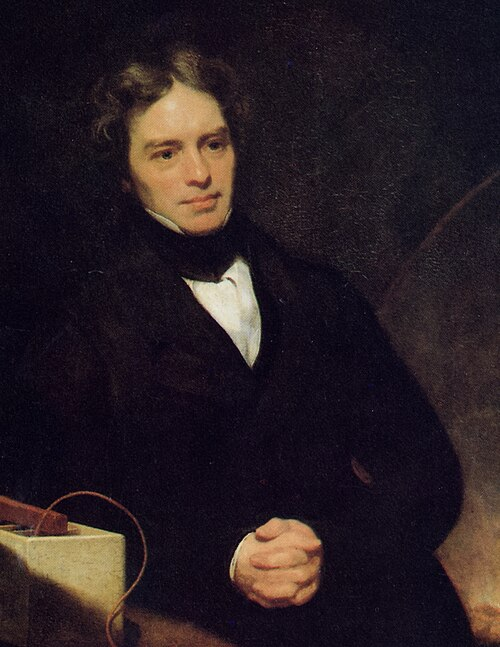
\includegraphics[width=\linewidth]{images/book3/faraday.jpg}
\end{minipage}\hfill
\begin{minipage}[t]{0.69\linewidth}
\vspace{0pt}
En 1834 Michael Faraday, midiendo los productos de electrólisis con un
voltámetro de su propio diseño, enunció que la masa de una sustancia producida
en un electrodo es proporcional a la cantidad de electricidad que ha pasado, y
que, para una cantidad de electricidad dada, las masas de las distintas sustancias
están en la razón de sus equivalentes químicos. Acuñó las palabras
electrodo, ánodo, cátodo, ion, anión y catión. La constante que lleva su
nombre convierte esas leyes en $Q = nF\,\Delta\xi$. (Retrato de Thomas Phillips,
1842, dominio público, Wikimedia Commons.)
\end{minipage}
\end{history}

\section{Pilas de concentración}

\begin{definition}[Pila de concentración]\label{def:b2:cell-thermodynamics:concentration-cell}
Una \emph{pila de concentración}\index{pila de concentracion@pila de concentración} está formada por dos
semipilas del mismo par que solo se diferencian en la concentración (o la
presión) de una especie.
\end{definition}

\begin{proposition}[Tensión de una pila de concentración]\label{prop:b2:cell-thermodynamics:concentration-cell}
Dos electrodos de un metal M sumergidos en disoluciones de \ce{M^{n+}} de
concentraciones $c_1 < c_2$, unidas por un puente salino, dan una tensión
\[
  U = \frac{RT}{nF}\ln\frac{c_2}{c_1} ,
\]
siendo el polo positivo el lado más concentrado. La pila funciona hasta que
las dos concentraciones se igualan.
\end{proposition}

\begin{proof}
Por la ecuación de Nernst, cada electrodo tiene $E_i = E^\circ + (RT/nF)\ln c_i$ (disoluciones
diluidas ideales); $E^\circ$ se cancela en la diferencia. La reacción es
\ce{M^{n+}}(lado 2) $\to$ \ce{M^{n+}}(lado 1): se deposita metal en el
lado concentrado (cátodo) y se disuelve en el lado diluido (ánodo), lo que
iguala las concentraciones; $\Delta_r G = RT\ln(c_1/c_2) < 0$ hasta que son
iguales.
\end{proof}

\begin{omfigure}
\begin{tikzpicture}[font=\small, >={Stealth}]
  \pic at (0,0) {beaker={0.7}{omDef!10}};
  \pic at (3.6,0) {beaker={0.7}{omDef!32}};
  \pic at (-0.3,0.25) {electrode={black!25}};
  \pic at (3.9,0.25) {electrode={black!25}};
  \pic at (0.35,0.55) {saltbridge={2.9}};
  \pic (m) at (1.8,4.3) {meter={V}};
  % common (black) terminal on the anode side, red (+) on the cathode side
  \fill[black] (1.4,4.03) circle (0.065); \fill[red!70!black] (2.2,4.03) circle (0.065);
  \draw[thick] (-0.15,2.65) |- (m-a);
  \draw[thick] (4.05,2.65) |- (m-b);
  \node[anchor=east] at (-0.95,1.0) {\ce{Ag}};
  \node[anchor=west] at (4.45,1.0) {\ce{Ag}};
  \node at (0.25,-0.35) {\ce{Ag+} \qty{0.010}{mol/L}};
  \node at (3.6,-0.35) {\ce{Ag+} \qty{0.10}{mol/L}};
  \node[anchor=east] at (-0.9,2.3) {$-$ ánodo};
  \node[anchor=west] at (4.6,2.3) {cátodo $+$};
  \node[font=\scriptsize] at (-0.1,-0.8) {\ce{Ag -> Ag+ + e-}};
  \node[font=\scriptsize] at (3.7,-0.8) {\ce{Ag+ + e- -> Ag}};
  \node[font=\scriptsize] at (1.8,5.05) {$U = \qty{59}{mV}$};
\end{tikzpicture}

{\small Una \omterm{def:b2:cell-thermodynamics:concentration-cell}{pila de concentración} de plata a \qty{25}{\degreeCelsius}. El lado diluido es
el ánodo: allí se disuelve plata, que se deposita en el lado concentrado,
hasta que las dos concentraciones se igualan. $U = 0.0592\log(0.10/0.010) =
\qty{59}{mV}$.}
\end{omfigure}

El mismo principio sirve para medir concentraciones. Un electrodo de vidrio, cuya fina
membrana separa una disolución de referencia de la muestra, desarrolla un potencial de membrana
de $(RT/F)\ln 10 = \qty{59}{mV}$ por unidad de diferencia de pH a
\qty{25}{\degreeCelsius}: el pHmetro del volumen del primer año es una \omterm{def:b2:cell-thermodynamics:concentration-cell}{pila de concentración}
para \ce{H+}. A través de la membrana de una célula viva, las concentraciones desiguales
de \ce{K+} crean del mismo modo un potencial de varias decenas de milivoltios.

\section{Ejercicios}

\begin{exercise}[$\star$]\label{exo:b2:cell-thermodynamics:1}
A partir de $\Delta_f G^\circ(\ce{H2O}, \text{l}) = \qty{-237.14}{kJ/mol}$, calcúlese la
tensión estándar de la pila hidrógeno--oxígeno.
\end{exercise}

\begin{exercise}[$\star$]\label{exo:b2:cell-thermodynamics:2}
Una batería tiene una capacidad nominal de \qty{1.0}{A.h}. Calcúlense la carga que contiene, en culombios,
y la masa de cinc consumida en su ánodo (\ce{Zn -> Zn^2+ + 2e-}) cuando está
completamente descargada.
\end{exercise}

\begin{exercise}[$\star$]\label{exo:b2:cell-thermodynamics:3}
Una pila Daniell da \qty{1.10}{V} sin corriente. Calcúlense $\Delta_r G$ para un
mol de cinc y el trabajo eléctrico máximo para \qty{10.0}{g} de cinc.
\end{exercise}

\begin{exercise}[$\star$]\label{exo:b2:cell-thermodynamics:4}
Dos electrodos de cobre se sumergen en disoluciones de sulfato de cobre(II) de \qty{1.0e-3}{mol/L}
y \qty{0.10}{mol/L}. Calcúlese la tensión a \qty{25}{\degreeCelsius} y nómbrense los
polos.
\end{exercise}

\begin{exercise}[$\star\star$]\label{exo:b2:cell-thermodynamics:5}
Una pila ($n = 2$) tiene $E^\circ = \qty{1.015}{V}$ y $dE^\circ/dT = \qty{-4.0e-4}{V/K}$
a \qty{298}{K} (datos del ejercicio). Calcúlense $\Delta_r G^\circ$, $\Delta_r S^\circ$ y
$\Delta_r H^\circ$.
\end{exercise}

\begin{exercise}[$\star\star$]\label{exo:b2:cell-thermodynamics:6}
La pila del \cref{exo:b2:cell-thermodynamics:5} descarga un mol de reacción
(a) de forma reversible; (b) a \qty{0.90}{V}. Calcúlense en cada caso el trabajo eléctrico y
el calor intercambiado con el entorno.
\end{exercise}

\begin{exercise}[$\star\star$]\label{exo:b2:cell-thermodynamics:7}
Calcúlese $E^\circ(\ce{Fe^3+}/\ce{Fe})$ a partir de las \omterm{def:b2:reaction-free-energy:gibbs-energy}{energías de Gibbs} de formación
(\ce{Fe^2+} \qty{-78.90}{kJ/mol}, \ce{Fe^3+} \qty{-4.7}{kJ/mol}) y compruébese que
es igual a $(E_1^\circ + 2E_2^\circ)/3$.
\end{exercise}

\begin{exercise}[$\star\star$]\label{exo:b2:cell-thermodynamics:8}
Calcúlese el potencial estándar del par \ce{AgCl}/\ce{Ag} y, después, el
potencial de un electrodo de cloruro de plata sumergido en cloruro de potasio de
\qty{0.10}{mol/L}.
\end{exercise}

\begin{exercise}[$\star\star$]\label{exo:b2:cell-thermodynamics:9}
Las pilas de cinc--aire usan \ce{2Zn + O2 -> 2ZnO} ($\Delta_f G^\circ(\ce{ZnO}) =
\qty{-318.30}{kJ/mol}$). Calcúlense la tensión estándar y la energía eléctrica
máxima, en \unit{kW.h}, por kilogramo de cinc.
\end{exercise}

\begin{exercise}[$\star\star\star$]\label{exo:b2:cell-thermodynamics:10}
Una pila de combustible de metanol directo funciona con \ce{CH3OH(l) + 3/2O2 -> CO2 + 2H2O(l)}. A partir de
$\Delta_f H^\circ$ (\unit{kJ/mol}): \ce{CH3OH(l)} $-239$, \ce{CO2} $-393.51$,
\ce{H2O(l)} $-285.83$; y de $S^\circ$ (\unit{J/(K.mol)}): \ce{CH3OH(l)} 127.2,
\ce{CO2} 213.8, \ce{H2O(l)} 69.95, \ce{O2} 205.15, calcúlense $n$, $E^\circ$ y el
rendimiento máximo.
\end{exercise}

\begin{exercise}[$\star\star\star$]\label{exo:b2:cell-thermodynamics:11}
Una pila ($n = 2$) tiene $E = \qty{0.500}{V}$ y $dE/dT = \qty{+3.0e-4}{V/K}$ a
\qty{298}{K} (datos del ejercicio). Demuéstrese que, funcionando de forma reversible, suministra más
trabajo eléctrico que $-\Delta_r H$, y explíquese de dónde procede la energía extra.
\end{exercise}

\begin{exercise}[$\star\star\star$]\label{exo:b2:cell-thermodynamics:12}
Dos electrodos de hidrógeno (\qty{1}{bar} de \ce{H2}) se sumergen en una disolución de referencia de
pH 7.00 y en una muestra. La tensión es de \qty{0.177}{V} a \qty{25}{\degreeCelsius},
siendo la referencia el polo positivo. Hállese el pH de la muestra, y explíquese
por qué el resultado no depende de ningún potencial estándar.
\end{exercise}

\section{Problema: el autobús de pila de combustible}

\begin{problem}[{Problema de fin de semana --- la tensión estándar de la pila
hidrógeno--oxígeno a partir de las energías de Gibbs, su coeficiente de temperatura, el
rendimiento y el calor de una pila real y la energía de un depósito de hidrógeno}]
\label{pb:b2:cell-thermodynamics:1}
Una pila de combustible tiene 400 celdas en serie, cada una con una membrana de
intercambio de protones (electrolito ácido). Datos a \qty{298.15}{K} (CODATA, JANAF):
$\Delta_f H^\circ(\ce{H2O}, \text{l}) = \qty{-285.83}{kJ/mol}$, $\Delta_f
G^\circ(\ce{H2O}, \text{l}) = \qty{-237.14}{kJ/mol}$, $\Delta_f G^\circ(\ce{H2O},
\text{g}) = \qty{-228.58}{kJ/mol}$; $S^\circ$ (\unit{J/(K.mol)}): \ce{H2O(l)} 69.95,
\ce{H2} 130.68, \ce{O2} 205.15. $F = \qty{96485}{C/mol}$; $M(\ce{H2}) =
\qty{2.016}{g/mol}$.
% ledger: dfh:H2O-l, janafG:H2O_l.298, janafG:H2O.298, s0:H2O_l, s0:H2_g, s0:O2_g, const:F, aw:H

\medskip
\noindent\textbf{Parte I --- La tensión estándar.}
\begin{enumerate}
  \item Escríbanse las semirreacciones en el ánodo y en el cátodo, y la reacción de
        la pila.
  \item ¿Cuántos electrones se intercambian por molécula de hidrógeno?
  \item Calcúlese $E^\circ$ cuando el agua se forma líquida.
  \item Calcúlese cuando el agua sale como vapor.
  \item Explíquese la diferencia con la \omterm{def:b2:reaction-free-energy:gibbs-energy}{energía de Gibbs} de vaporización del agua.
  \item Calcúlense $\Delta_r H^\circ$ y el rendimiento máximo a \qty{298}{K}.
\end{enumerate}

\medskip
\noindent\textbf{Parte II --- La temperatura.}
\begin{enumerate}[resume]
  \item Calcúlese $\Delta_r S^\circ$ para el agua líquida.
  \item Dedúzcase $dE^\circ/dT$.
  \item Estímese $E^\circ$ a \qty{80}{\degreeCelsius}, la temperatura de trabajo de la
        pila.
  \item Compárese el método con el valor JANAF a \qty{400}{K}, $\Delta_f
        G^\circ(\ce{H2O}, \text{l}) = \qty{-221.01}{kJ/mol}$.
  \item ¿Qué calor intercambia la pila reversible por mol de hidrógeno a
        \qty{298}{K}? ¿Lo recibe o lo cede?
  \item Estímese el rendimiento máximo a \qty{80}{\degreeCelsius}.
\end{enumerate}

\medskip
\noindent\textbf{Parte III --- La pila real a \qty{0.70}{V} por celda.}
\begin{enumerate}[resume]
  \item Calcúlese el trabajo eléctrico por mol de hidrógeno.
  \item Calcúlese el rendimiento referido a $\Delta_r H^\circ$ y a $\Delta_r G^\circ$.
  \item Calcúlese el calor liberado por mol de hidrógeno.
  \item ¿Qué parte es inevitable, y qué parte se debe a la corriente?
  \item La pila suministra \qty{300}{A}. Calcúlese el consumo de hidrógeno de una
        celda y luego de la pila completa, en moles y en gramos por segundo.
  \item Calcúlese la potencia eléctrica de la pila.
  \item Calcúlese la potencia térmica que debe evacuar el circuito de refrigeración.
\end{enumerate}

\medskip
\noindent\textbf{Parte IV --- El depósito.}
\begin{enumerate}[resume]
  \item ¿Qué cantidad de hidrógeno hay en \qty{5.0}{kg}?
  \item ¿Qué carga pasa por las celdas, contada sobre todas ellas, cuando
        se oxida este hidrógeno?
  \item Calcúlese la energía eléctrica suministrada por la pila, con cada celda a
        \qty{0.70}{V}.
  \item Conviértase en kilovatios hora.
  \item ¿Durante cuánto tiempo puede la pila suministrar la potencia de la pregunta 18?
  \item Indíquese la energía eléctrica que suministran \qty{5.0}{kg} de hidrógeno a
        \qty{0.70}{V} por celda.
\end{enumerate}
\end{problem}
